\documentclass[CJK]{beamer}
\usepackage{CJKutf8}
\usepackage{beamerthemesplit}
\usetheme{Malmoe}
\useoutertheme[footline=authortitle]{miniframes}
\usepackage{amsmath}
\usepackage{amssymb}
\usepackage{graphicx}
\usepackage{color}
\usepackage{slashed}
\usepackage{simplewick}
\graphicspath{{../figures/}}
\def\be{\begin{equation}}
\def\ee{\nonumber\end{equation}}
\def\bea{\begin{eqnarray}}
\def\eea{\nonumber\end{eqnarray}}
\def\ii{{\dot{\imath}}}
\def\bch{\begin{CJK}{UTF8}{gbsn}}
\def\ech{\end{CJK}}
\def\bex{\begin{minipage}{0.3\textwidth}
\includegraphics[width=1in]{jugelizi.png}\end{minipage}\begin{minipage}{0.6\textwidth}}
\def\eex{\end{minipage}}
\def\chtitle#1{\frametitle{\bch#1\ech}}
\def\skipline{{\vskip0.1in}}
\def\skiplines{{\vskip0.2in}}
\def\lagr{{\mathcal{L}}}
\def\hamil{{\mathcal{H}}}
\def\vecv{{\mathbf{v}}}
\def\vecx{{\mathbf{x}}}
\def\veck{{\mathbf{k}}}
\def\vecp{{\mathbf{p}}}
\def\vecn{{\mathbf{n}}}
\def\vecA{{\mathbf{A}}}
\def\vecP{{\mathbf{P}}}
\def\vecsigma{{\mathbf{\sigma}}}
\def\hatJn{{\hat{J_\vecn}}}
\def\hatJx{{\hat{J_x}}}
\def\hatJy{{\hat{J_y}}}
\def\hatJz{{\hat{J_z}}}
\def\hatj#1{\hat{J_{#1}}}
\def\hatphi{{\hat{\phi}}}
\def\hatq{{\hat{q}}}
\def\hatpi{{\hat{\pi}}}
\def\vel{\upsilon}
\def\Dint{{\mathcal{D}}}
\def\adag{{\hat{a}^\dagger}}
\def\bdag{{\hat{b}^\dagger}}
\def\cdag{{\hat{c}^\dagger}}
\def\ddag{{\hat{d}^\dagger}}
\def\hata{{\hat{a}}}
\def\hatb{{\hat{b}}}
\def\hatc{{\hat{c}}}
\def\hatd{{\hat{d}}}
\def\hatN{{\hat{N}}}
\def\hatH{{\hat{H}}}
\def\hatp{{\hat{p}}}
\def\Fup{{F^{\mu\nu}}}
\def\Fdown{{F_{\mu\nu}}}
\def\newl{\nonumber \\}
\def\SIkm{\mathrm{km}}
\def\SIyr{\mathrm{yr}}
\def\SIGyr{\mathrm{Gyr}}
\def\SIeV{\mathrm{eV}}
\def\SIGeV{\mathrm{GeV}}
\def\SIm{\mathrm{m}}
\def\SIcm{\mathrm{cm}}
\def\SIJ{\mathrm{J}}
\def\SIs{\mathrm{s}}
\def\SIkg{\mathrm{kg}}
\def\SIg{\mathrm{g}}
\def\vece{\mathrm{e}}
\def\bmat#1{\left(\begin{array}{#1}}
\def\emat{\end{array}\right)}
\def\bcase#1{\left\{\begin{array}{#1}}
\def\ecase{\end{array}\right.}
\def\calM{{\mathcal{M}}}
\def\calT{{\mathcal{T}}}
\def\calR{{\mathcal{R}}}
\def\barpsi{\bar{\psi}}
\def\baru{\bar{u}}
\def\barv{\bar{\upsilon}}
\def\bmini#1{\begin{minipage}{#1\textwidth}}
\def\emini{\end{minipage}}
\def\qeq{\stackrel{?}{=}}
\def\torder#1{\mathcal{T}\left(#1\right)}
\def\rorder#1{\mathcal{R}\left(#1\right)}


\title{Quantum Field Theory I \\ Lesson 16 - QED Introduction}
\author{}
\date{}


\begin{document}

\begin{frame}
 
\begin{center}
\begin{Large}
\bch
量子场论 I 

{\vskip 0.3in}

第十六课 量子电动力学(QED)初步介绍

\ech
\end{Large}
\end{center}

\vskip 0.2in

\bch
课件下载
\ech
https://github.com/zqhuang/SYSU\_QFTI

\end{frame}

\begin{frame}
\chtitle{Background}
\bch
自然界有四种基本作用力——引力,电磁力,强相互作用力和弱相互作用力。我们以前学过的电动力学是对电磁力的经典描述。量子电动力学(QED)则是对电磁力的量子描述,它是物理学里最严谨最精密的一个分支。
\skipline

QED研究的是自旋为$1/2$的Dirac场和自旋为$1$的$U(1)$规范场的相互作用。拉氏密度为:
$$\lagr = -\frac{1}{4}\Fup\Fdown + \bar\psi(\ii\slashed{D} - m)\psi$$
其中$D_\mu = \partial_\mu + iq A_\mu$, $q$为Dirac场粒子的电荷。
\ech
\end{frame}


\begin{frame}
\chtitle{定域规范不变性}
\bch
证明QED在定域规范变换
$$A_\mu \rightarrow A_\mu - \frac{1}{q}\partial_\mu \gamma$$
$$\psi \rightarrow \psi e^{\ii  \gamma}$$
下作用量不变。

\ech
\end{frame}


\begin{frame}
\chtitle{场方程}
\bch
试推导QED的场方程:
$$(\ii\slashed{D} - m)\psi = 0$$
和
$$\partial_\mu \Fup = j^\nu \equiv q \barpsi \gamma^\nu \psi$$
\ech
\end{frame}

\begin{frame}
\chtitle{电荷守恒}
\bch
显然
$$j^\nu \equiv q \barpsi \gamma^\nu \psi$$
是守恒流(可以直接用上面的场方程证明或者用全局规范对称性和Noether定理来证明),
$$ Q = \int d^3\vecx\, j^0  = q\int d^3\vecx\,\barpsi \gamma^0\psi $$
是守恒电荷。
\ech
\end{frame}

\begin{frame}
\chtitle{QED的相互作用绘景}
\bch

在$A_0 = 0$, $\nabla\cdot \vecA = 0$的规范下,
$$\lagr = \frac{1}{2}\left(|\dot{\vecA}|^2 - |\nabla\times \vecA|^2\right) + \barpsi(i\slashed{\partial}-m)\psi - q\bar\psi\slashed{A}\psi$$


我们仍然把自由场的Hamilton量作为$\hatH_0$,相互作用Hamilton量为
$$\hatH_I = \int d^3\vecx\, A_\mu j^\mu = q \int d^3\vecx\, \barpsi\slashed{A}\psi$$


\ech
\end{frame}

\begin{frame}
\chtitle{热身问题:Compton散射}
\bch
{\small
QED里最简单的问题是Compton散射问题:一个电子和一个光子发生碰撞,变成不同动量的电子和光子。
\skipline

设电子和光子的动量初态为$p_e$和$p_\gamma$,末态为$p_e'$和$p_\gamma'$。因为现在相互作用为两个$\psi$和一个$\vecA$, 最简单的Feynman图就长这样:
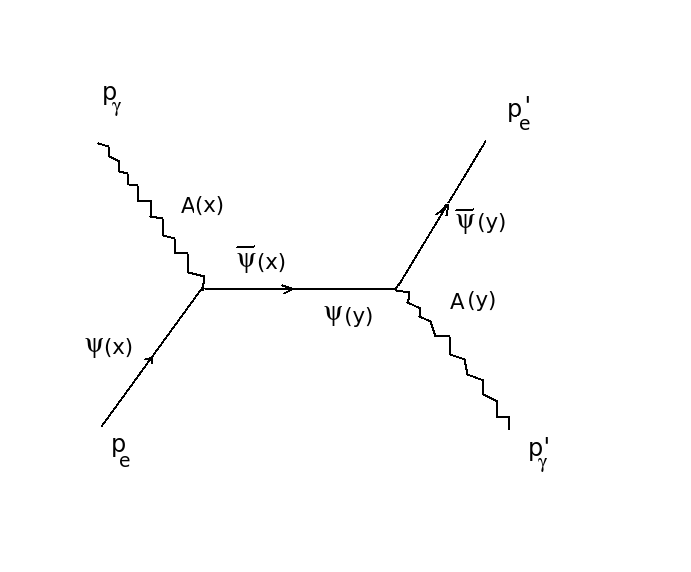
\includegraphics[width=1.8in]{feynman3_s.png}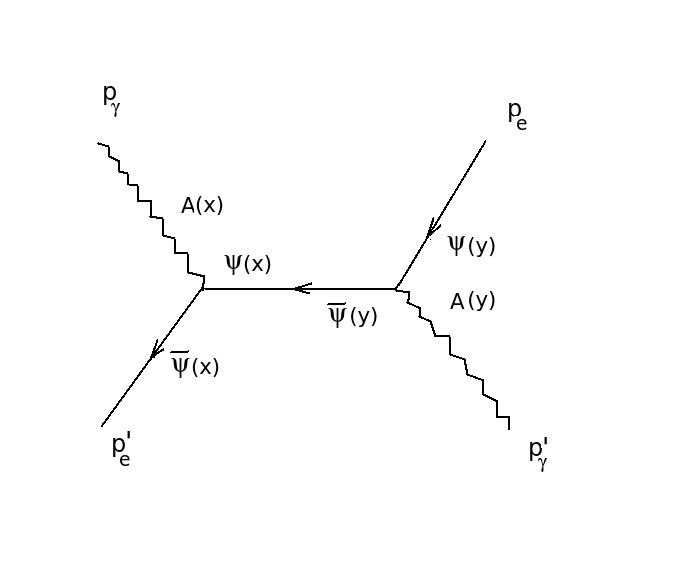
\includegraphics[width=1.8in]{feynman3_u.png}

再加上$x$,$y$互换,每个图要乘以2,恰好和泰勒展开中的$1/(2!)$抵消。注意对固定的电子(正粒子), $\hat\psi$只包含湮灭算符,$\hat{\barpsi}$只包含产生算符。所以图中的$\barpsi$和$\psi$不能随意交换次序。}
\ech
\end{frame}


\begin{frame}
\chtitle{Feynman传播子}
\bch
为了计算QED的Feynman图,我们先计算Feynman传播子
$$\contr{\hat\psi(x)}{\hat{\barpsi}(y)}$$
同样它也可以看成自由$\psi$场的关联矩阵的矩阵元。自由$\psi$场的关联矩阵为
$$ \ii\left(\ii \slashed{\partial}-m + \ii\epsilon\right)^{-1} \rightarrow \frac{\ii}{\slashed{k} - m + \ii\epsilon}$$
在傅立叶空间计算矩阵元:
$$\contr{\hat\psi(x)}{\hat{\barpsi}(y)} = \frac{1}{(2\pi)^4}\int d^4k\, \frac{\ii e^{-\ii k(x-y)}}{\slashed{k} - m + \ii\epsilon} $$
当然,我们希望能绕开这些积分过程直接用Feynman规则进行计算。体积元$d^3\vecp$和$e^{-\ii px}$等的组合最后都会给出正确的$T/V\delta(p_\gamma+p_e - p_\gamma'-p_e')d^4k$因子,所以我们在推导Feynman规则时不再关注它们。
\ech
\end{frame}

\begin{frame}
\chtitle{其他几条Feynman规则}
\bch
{\small
\begin{itemize}
\item{顶点给出因子$-\ii q \gamma^\mu$}
\item{电子内线给出Feynman传播子$\frac{\ii}{\slashed{k}-m}$}
\item{对于一个初态的动量为$\vecp$,自旋为$s$的电子外线,我们需要从$\hat\psi$中提取一个湮灭算符$\hata_{\vecp,s}$,对应的系数为$u_{\vecp, s}$。}
\item{对于一个末态的电子外线,则需要提取产生算符$\hat{\barpsi}$里的$\adag_{\vecp,s}$,随之带来的因子为$\bar{u}_{\vecp,s}$。}
\item{初态的光子对应的因子为$\vece^\mu_{\vecp,s}/\sqrt{2\omega}$。这里的$\mu$为跟它连接的顶点的$-iq\gamma^\mu$里的指标$\mu$。}
\item{末态的光子对应的因子为${\vece^\mu_{\vecp,s}}^*/\sqrt{2\omega}$。这里的$\mu$为跟它连接的顶点的$-iq\gamma^\mu$里的指标$\mu$。}
\end{itemize}

{\scriptsize
注:

1. 如果是反粒子则把$u$换成$\upsilon$。

2. 在库仑规范下矢量$\vece$第0分量为零。} 

}

\ech
\end{frame}

\begin{frame}
\chtitle{第一个图}
\bch
{\small
\bmini{0.5}
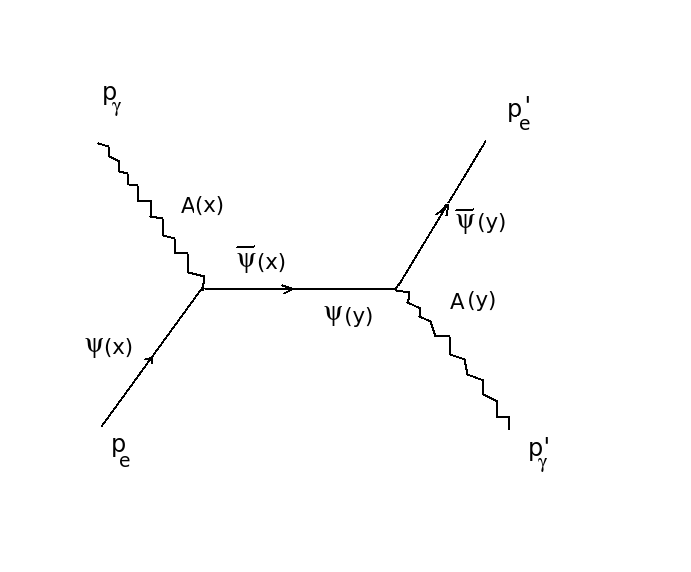
\includegraphics[width=2in]{feynman3_s.png}
\emini
\bmini{0.4}
 + ($x$, $y$ 互换)
\emini
\be
= \frac{(-\ii q)^2}{2\sqrt{\omega_\gamma\omega_\gamma'}}\sum_{s_e, s_\gamma, s_e', s_\gamma'} \bar{u}_{p_e',s'_e} \slashed{\vece}^*_{p_\gamma',s_\gamma'}\frac{\ii}{\slashed{p}_e+\slashed{p}_\gamma-m}\slashed{\vece}_{p_\gamma,s_\gamma} u_{p_e,s_e}  
\ee
}
\ech
\end{frame}

\begin{frame}
\chtitle{第二个图}
\bch
{\small
\bmini{0.5}
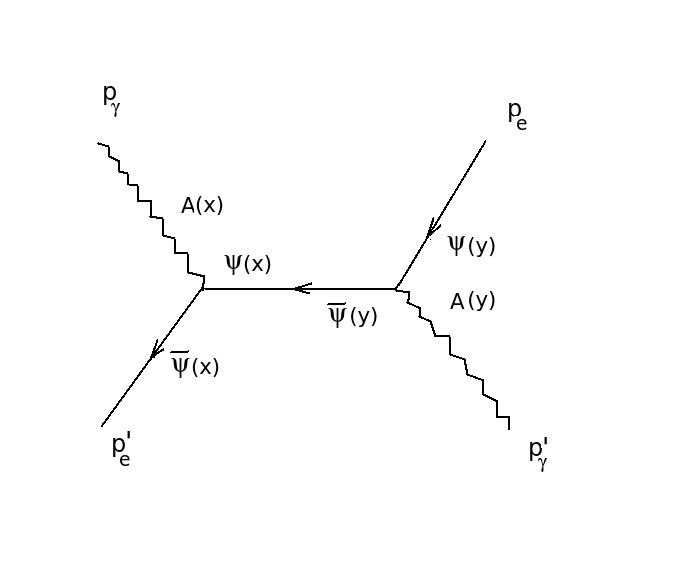
\includegraphics[width=2in]{feynman3_u.png}
\emini
\bmini{0.4}
 + ($x$, $y$ 互换)
\emini
\be
= \frac{(-\ii q)^2}{2\sqrt{\omega_\gamma\omega_\gamma'}}\sum_{s_e, s_\gamma, s_e', s_\gamma'} \bar{u}_{p_e',s'_e} \slashed{\vece}^*_{p_\gamma',s_\gamma'}\frac{\ii}{\slashed{p}_e-\slashed{p}_\gamma'-m}\slashed{\vece}_{p_\gamma,s_\gamma} u_{p_e,s_e}  
\ee
}
\ech
\end{frame}

\begin{frame}
\chtitle{世界上最遥远的距离,就是Feynman图和最终结果之间的距离}
\bch

我们需要计算总散射截面的绝对值的平方:
{\scriptsize
\be
 |\calM|^2 = \frac{q^4}{4 \omega_\gamma\omega_\gamma'} \left\vert\sum_{s_e, s_\gamma, s_e', s_\gamma'}\bar{u}_{p_e',s'_e} \slashed{\vece}^*_{p_\gamma',s_\gamma'}\left(\frac{\ii}{\slashed{p}_e+\slashed{p}_\gamma-m}+\frac{\ii}{\slashed{p}_e-\slashed{p}_\gamma'-m}\right)\slashed{\vece}_{p_\gamma,s_\gamma} u_{p_e,s_e}   \right\vert^2
\ee
}

只要十来页纸的计算就能把上式化简到最后结果,但今天我们比较忙,这点小事先放一放,来聊点别的。
\ech
\end{frame}

\begin{frame}
\chtitle{最后一条Feynman规则}
\bch
先撇开那些令人赏心悦目(sh\={e}ng b\`{u} r\'{u} s\v{i})的计算不说,我们还差最后一条Feynman规则没讨论。如果初态和末态都是Dirac费米子,那么我们需要把两个$A$收缩掉。对应的Feynman图长成这样:

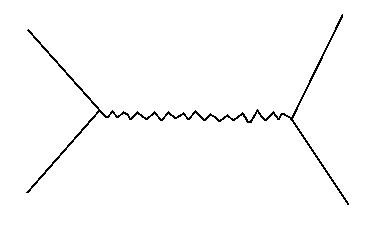
\includegraphics[width=2.5in]{feynman4_sketch.png}

\ech
\end{frame}

\begin{frame}
\chtitle{最后一条Feynman规则}
\bch
我们还是用直接写出矩阵元的方法。
在洛仑兹规范下写出傅立叶空间的拉氏密度:
$$\ii\lagr = -\frac{1}{2}A_\mu (C^{-1})_{\mu\nu} A_\nu$$ 
其中
$$C_{\mu\nu} = \lim_{\epsilon\rightarrow 0^+}\frac{-\ii g_{\mu\nu}}{k^2+\ii\epsilon}$$
于是有了最后一条Feynman规则:
\begin{itemize}
\item{光子内线对应的$\frac{-\ii g_{\mu\nu}}{k^2}$,其中的$\mu$, $\nu$为跟它连接的两个顶点的指标(即这两个顶点分别为$-\ii q\gamma^\mu$和$-\ii q \gamma^\nu$)。}
\end{itemize}

\ech
\end{frame}


\begin{frame}
\bch
下节课我们讲那些计算的小事。
\ech
\end{frame}

\end{document}


